\documentclass[a4paper]{article}
\usepackage{amsfonts}
\usepackage{amsmath}
\usepackage{amssymb}
\usepackage{graphicx}     
\usepackage[a4paper,landscape]{geometry}    

\begin{document}
  
\noindent \large Auteur: Sabawoon Enayat      \\
\noindent \large Studierichting: Informatica  \\
\noindent \large Oefeningenreeks 3G nr. 4 \\

\newcommand{\llim}{\lim\limits}

\medskip

\normalsize

Opgave: $f(x) = x^4 - 4x^4 = x^2 (x^2 - 4)$\\

$\operatorname{dom}f = \mathbb{R} \Rightarrow$ geen VA\\

$f^{-1}(0) = \left\{-2, 0^{(2)}, 2\right\}$\\

$\llim_{x\to\infty} f(x) = \infty \Rightarrow$ geen HA\\

$gr(T) \ne gr(N) + 1$ en $\llim_{x\to\infty} \dfrac{f(x)}{x} = \infty \Rightarrow$ geen SA\\

$f'(x) = 4x^3 - 8x = 4x\left(x^2 - 2\right)$\\

$(f')^{-1}(0) = \left\{-\sqrt{2}, 0, \sqrt{2}\right\}$\\

$f''(x) = 12x^2 - 8$\\

$(f'')^{-1}(0) = \left\{\dfrac{-\sqrt{6}}{3}, \dfrac{\sqrt{6}}{3}\right\}$\\

\begin{tabular}{c|ccccccccccccccccc}
	$x$      & $-\infty$ &  & $-2$ &  & $-\sqrt{2}$ &  & $\dfrac{-\sqrt{6}}{3}$ &  & $0$ &  & $\dfrac{\sqrt{6}}{3}$ &  & $\sqrt{2}$ & & $2$ & & $+\infty$ \\ \hline 
	$f(x)$   & $-\infty$ & $+$ & $0$ & $-$ & $-$ & $-$ & $-$ & $-$ & $0^{(2)}$ & $-$ & $-$ & $-$ & $-$ & $-$ & $0$ & $+$ & $+\infty$ \\ 
	$f'(x)$  & $-$ & $-$ & $-$ & $-$ & $0$ & $+$ & $+$ & $+$ & $0$ & $-$ & $-$ & $-$ & $0$ & $+$ & $+$ & $+$ & $+$\\
	$f''(x)$ & $+$ & $+$ & $+$ & $+$ & $+$ & $+$ & $0$ & $-$ & $-$ & $-$ & $0$ & $+$ & $+$ & $+$ & $+$ & $+$ & $+$ \\ \hline
	$f(x)$ & $\searrow$ & $\searrow$ & $\searrow$ & $\searrow$ & $m(-4)$ & $\nearrow$ & $\nearrow$ & $\nearrow$ & $M(0)$ & $\searrow$ & $\searrow$ & $\searrow$ & $m(-4)$ & $\nearrow$ & $\nearrow$ & $\nearrow$ & $\nearrow$ \\
		   & $\smile$ & $\smile$ & $\smile$ & $\smile$ & $\smile$ & $\smile$ & $B\left(-\dfrac{20}{9}\right)$ & $\frown$ & $\frown$ & $\frown$ & $B\left(-\dfrac{20}{9}\right)$ & $\smile$ & $\smile$ & $\smile$ & $\smile$ & $\smile$ & $\smile$ \\
\end{tabular} \\

$f\left(\sqrt{2}\right) = -4$\\

$f\left(\dfrac{\sqrt{6}}{3}\right) = \dfrac{-20}{9}$\\

\begin{figure}[h]
	\centering
	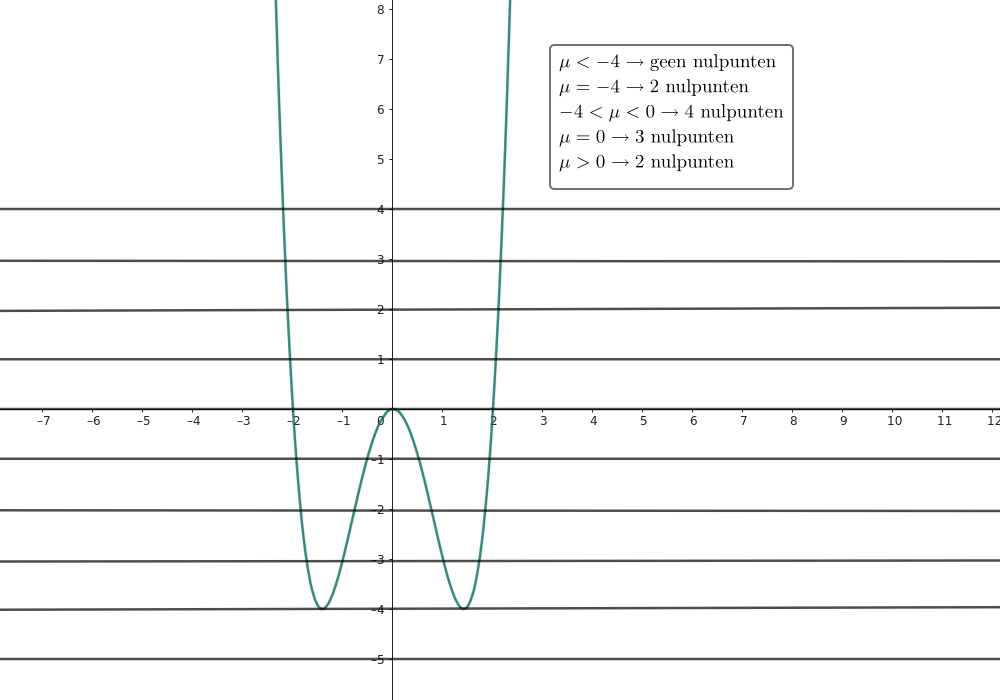
\includegraphics[width=15cm]{3G-4-sabawoon.enayat.INF.png}
\end{figure}

\begin{thebibliography}{999}
%\bibitem{a} Referentie
\end{thebibliography}
\end{document} 
